\documentclass[tikz,border=2pt]{standalone}
\usepackage{amsmath,amssymb}
\usetikzlibrary{arrows.meta,positioning,shapes,fit,calc}

\begin{document}
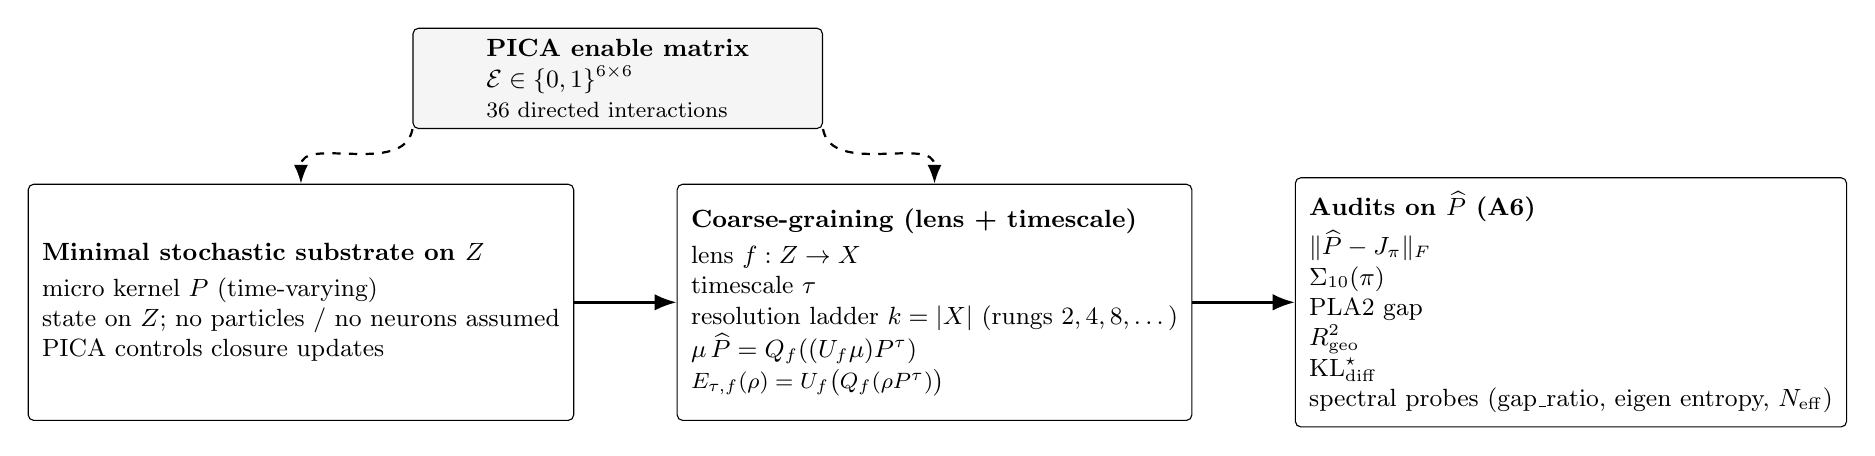
\begin{tikzpicture}[
  font=\small,
  node distance=11mm and 9mm,
  box/.style={draw, rounded corners=2pt, align=left, inner sep=5pt},
  ctrl/.style={draw, rounded corners=2pt, align=left, inner sep=4pt, fill=gray!8},
  flow/.style={-{Latex[length=2.8mm]}, line width=0.9pt},
  ctl/.style={-{Latex[length=2.4mm]}, line width=0.8pt, dashed}
]

% Main boxes
\node[box, minimum width=4.9cm, minimum height=3.0cm] (micro) {
\textbf{Minimal stochastic substrate on $Z$}\\[2pt]
micro kernel $P$ (time-varying)\\
state on $Z$; no particles / no neurons assumed\\
PICA controls closure updates
};

\node[box, right=13mm of micro, minimum width=5.9cm, minimum height=3.0cm] (coarse) {
\textbf{Coarse-graining (lens + timescale)}\\[2pt]
lens $f:Z\to X$\\
timescale $\tau$\\
resolution ladder $k=|X|$ (rungs $2,4,8,\dots$)\\
$\mu\,\widehat{P}=Q_f\!\left((U_f\mu)P^{\tau}\right)$\\
\footnotesize $E_{\tau,f}(\rho)=U_f\!\left(Q_f(\rho P^{\tau})\right)$
};

\node[box, right=13mm of coarse, minimum width=5.5cm, minimum height=3.0cm] (audit) {
\textbf{Audits on $\widehat{P}$ (A6)}\\[2pt]
$\|\widehat P - J_{\pi}\|_F$\\
$\Sigma_{10}(\pi)$\\
PLA2 gap\\
$R^2_{\mathrm{geo}}$\\
$\mathrm{KL}^{\star}_{\mathrm{diff}}$\\
spectral probes (gap\_ratio, eigen entropy, $N_{\mathrm{eff}}$)
};

% PICA control box — raised above box tops to avoid overlap
\node[ctrl, above=22mm of $(micro)!0.50!(coarse)$, minimum width=5.2cm] (pat) {
\textbf{PICA enable matrix}\\
$\mathcal{E}\in\{0,1\}^{6\times 6}$\\
\footnotesize 36 directed interactions
};

% Main flow
\draw[flow] (micro.east) -- (coarse.west);
\draw[flow] (coarse.east) -- (audit.west);

% PICA controls — arrows arrive vertically at box tops, clear of titles
\draw[ctl] (pat.south west) to[out=-100,in=90] (micro.north);
\draw[ctl] (pat.south east) to[out=-80,in=90] (coarse.north);

\end{tikzpicture}
\end{document}
